\section{Umsetzung}

\subsection{Interaktion mit dem Bitcoin Netzwerk}

Möchte man mit dem Bitcoin Netzwerk kommunizieren, benötigt man einen Client, der das Bitcoin Protokoll implementiert. Dieser interagiert mit dem Peer-to-Peer Netzwerk und wird dadurch zu einem Netzwerk-Knoten. Man unterscheidet zwischen sogenannten \textit{Full-Nodes} und \textit{Light-Nodes}.
\subsubsection{Full-Node}
Knoten die eigenständig alle Transaktionen und Blöcke auf Gültigkeit mit Hilfe der Konsensregeln prüfen, nennt man Full-Node. Diese Knoten speichern die gesamte Blockchain und bilden das Rückgrat des Netzwerks.
Full-Nodes stellen in der Regel eine RPC Schnittstelle zur Verfügung. Diese Schnittstelle bietet die Möglichkeit von einer beliebigen Programmiersprache aus mit dem Full-Node zu interagieren.
Abbildung \ref{fig:btc_core_full_node_architecture} zeigt, dass man über die RPC Schnittstelle auf die gespeicherten Daten des Nodes (Blöcke, Blockheader und Adressen) als auch auf die Wallet zugreifen kann.

\begin{figure}[H]
\centering
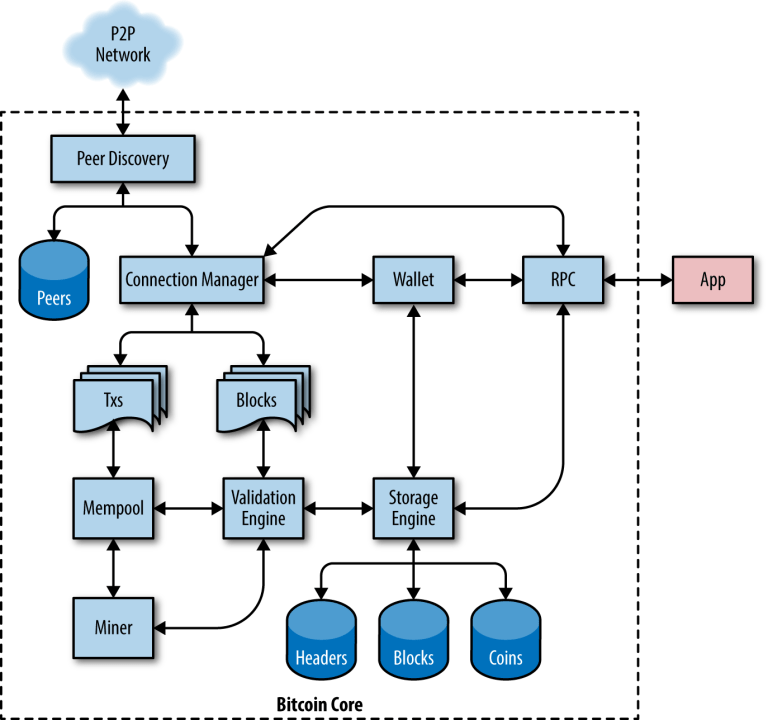
\includegraphics[width=1\linewidth]{Figures/btc_core_full_node_architecture}
\decoRule
\caption{Bitcoin Core: Full-Node Aufbau \cite{mastering_bitcoin}}
\label{fig:btc_core_full_node_architecture}
\end{figure}
Abbildung \ref{fig:btc_core_full_node_architecture} zeigt außerdem: 
\begin{itemize}
\item Peer Discovery, Peer Datenbank und Connection Manager: Diese kümmern sich um die Kommunikation mit dem Peer-to-Peer Netzwerk.
\item Mempool: Im sogenannten Mempool werden empfangene, unbestätigte Transaktionen im Speicher gehalten.
\item Validation Engine: Diese validiert, ob die empfangenen Blöcke und deren Transaktionen die Konsensregeln einhalten. Falls ja werden die somit bestätigten Transaktionen aus dem Mempool gelöscht und der Block wird an die StorageEngine zur Abspeicherung in der Blockchain Datenbank weitergereicht.
\item Miner: Die Bitcoin Full-Node Software enthält einen CPU Miner mit der man mithilfe des Proof-of-Work Algorithmus nach neuen Blöcken suchen kann. Bitcoin Mining ist heutzutage allerdings nur noch mit sogenannten ASICs profitabel. ASIC steht für \textbf{A}pplication-\textbf{S}pecific \textbf{I}ntegrated \textbf{C}ircuit. Es handelt sich um Hardware, die auf eine möglichst performante Berechnung der SHA256 Hashfunktion spezialisiert ist.
\end{itemize}


\subsubsection{Light-Node}
Light-Nodes speichern nicht die gesamte Blockchain, sonder in der Regel nur die Blockheader der Blöcke der Blockchain. Beim Mining gehen nur die Daten des Blockheaders in den Blockhash ein (siehe \ref{tab:btc_block_header}). Der Node empfängt Blockheader, prüft ihre Gültigkeit und fügt sie gegebenenfalls in die Headerkette ein. Der Node kann somit eigenständig, d.h. ohne seinen Nachbarn vertrauen zu müssen, die längste Proof-of-Work Kette bilden. Da diese Kette nur aus Headern besteht und keine Transaktionen enthält, kann der Light-Node empfangene Transaktionen nicht eigenständig auf ihre Gültigkeit prüfen. Light-Nodes verwenden das in \cite{bitcoin_white_paper} beschriebene \textbf{S}implified \textbf{P}ayment \textbf{V}erification Verfahren zur Prüfung von Transaktionen. Light-Nodes werden daher oft auch \textit{SPV-Client} genannt. Ein \textbf{SPV}-Client prüft die Gültigkeit einer Transaktion, indem er sie an der richtigen Stelle der Headerkette einordnet und dann den passenden Merkel-Branch von einem Full-Node anfragt. Durch diese Zusätzlichen Daten kann er nun wie in Abbildung \ref{fig:spv_chain} gezeigt nachprüfen, ob der Hash der Transaktion wirklich in den Wurzelknoten des Merkel-Trees mit eingegangen ist.

\begin{figure}[H]
\centering
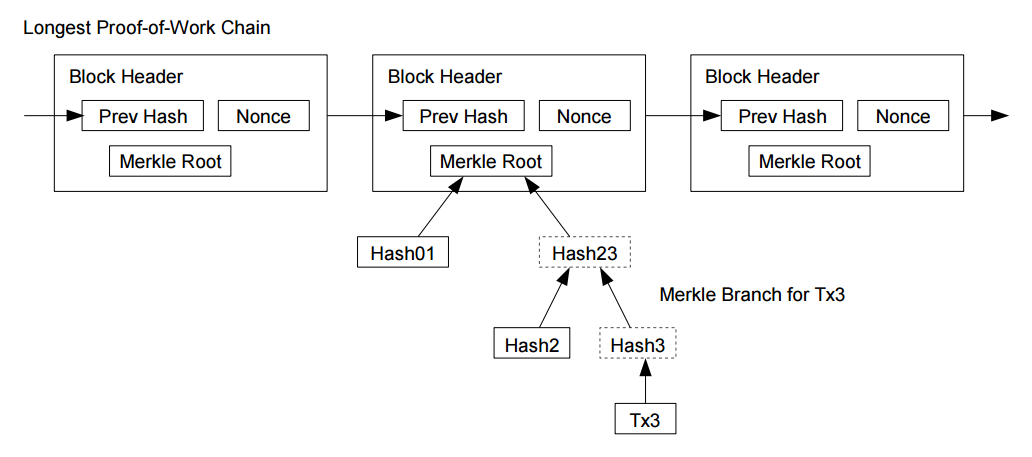
\includegraphics[width=1\linewidth]{Figures/umsetzung_btc/spv_chain}
\decoRule
\caption{Blockheader Kette \cite{ethereum_white_paper}}
\label{fig:spv_chain}
\end{figure}

Für den Bitcoin Teil dieser Ausarbeitung ist die Integration mit dem Peer-to-Peer Netzwerk mit Hilfe der in Java geschriebenen BitcoinJ \cite{bitcoinj} Bibliothek umgesetzt. Diese ermöglicht die Interaktion mit dem Netzwerk als SPV-Client.

\subsection{Überblick}

Abbildung \ref{fig:anwendung_aufbau} skizziert die Komponenten der Glücksspielanwendung und wie diese mit ihrer Umgebung kommunizieren. Es gibt zum einen den Server auf dem die Glücksspielanwendung läuft, die Spieler und das Bitcoin Netzwerk.

\begin{figure}[H]
\centering
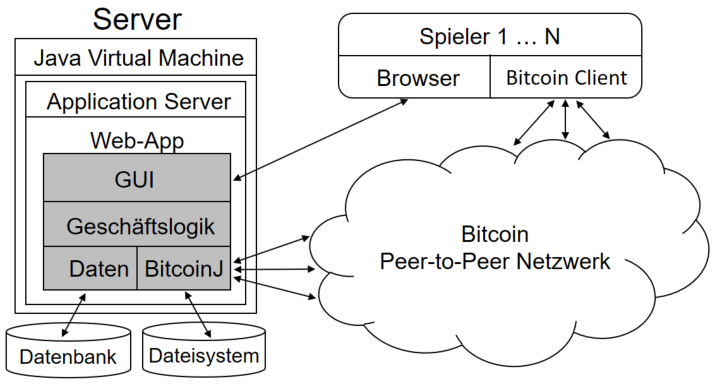
\includegraphics[width=1\linewidth]{Figures/umsetzung_btc/anwendung_aufbau}
\decoRule
\caption{Glücksspielanwendung Aufbau und Interaktion}
\label{fig:anwendung_aufbau}
\end{figure}

\subsubsection{Glücksspielanwedung}
\begin{itemize}
\item Server: Die Glücksspielanwendung läuft auf einem Server, der über eine Java Virtual Machine (JVM) Laufzeitumgebung verfügt, eine MySQL Datenbank und ein gewöhnliches Dateisystem besitzt.
\item Java Virtual Machine (JVM): Innerhalb der JVM läuft ein sogenannter Application Server, der eine Webanwendung nach außen bereitstellt. Auf diese Webanwendung können die Spieler über das HTTP Protokoll mittels ihres Browsers zugreifen. Die Webanwendung besteht aus mehreren Komponenten.
\item Application Server: Dieser stellt die Applikation bereit. Bei der Umsetzung der Glücksspielanwendung wurde der Open Source Application Server Wildfly\footnote{\url{http://wildfly.org/}} von der Firma Red Hat verwendet.
\item GUI: Die Weboberfläche stellt die zentrale Schnittstelle zwischen der Anwendung und dem Spieler da. Diese ist mithilfe des Tapestry\footnote{\url{http://tapestry.apache.org/}} Webframeworks von Apache umgesetzt. Detaillierte Informationen findet man in \cite{tapestry}.
\item Geschäftslogik: Diese behandelt sowohl die vom Benutzer über die GUI ausgelösten, als auch die vom Bitcoin Netzwerk ausgelösten Events.
\item BitcoinJ: Die Java Bibliothek, die zur Kommunikation mit dem Bitcoin Netzwerk verwendet wird.
\end{itemize}

\subsubsection{Spieler}
Die Spieler verfügen über einen Browser und über einen Bitcoin Client.
Mit dem Internetbrowser interagieren sie mit Glücksspielanwendung. Mit dem Bitcoin Client erstellen und empfangen sie Zahlungen.
\subsubsection{Bitcoin Peer-to-Peer Netzwerk}
Das Peer-to-Peer Netzwerk besteht aus den anderen Teilnehmern des Netzwerks. Dies sind Full-, Light-Nodes und Miner. Bei Kryptowährungsnetzwerken unterscheidet man in der Regel zwischen dem Test und Hauptnetzwerk. Den Bitcoins des Testnetzwerks wird kein monetärer Wert zugeschrieben. Das Testnetzwerk dient dazu Software, die mit dem Bitcoin Netzwerk interagieren soll, zu testen. Möchte ein Händler Bitcoin in seinen Onlineshop integrieren, kann er so seine Implementierung testen, ohne ein finanzielles Risiko einzugehen. 

\subsection{Datenmodel}
Die Klasse \code{Pot} repräsentiert ein Spiel und speichert alle für das Spiel relevanten Daten. Sie besteht aus einer Liste von Teilnehmern (\code{Participant}). Jeder Teilnehmer besitzt, wie im Konzept beschrieben, eine Ein- und Auszahlungsadresse.
\begin{figure}[H]
\centering
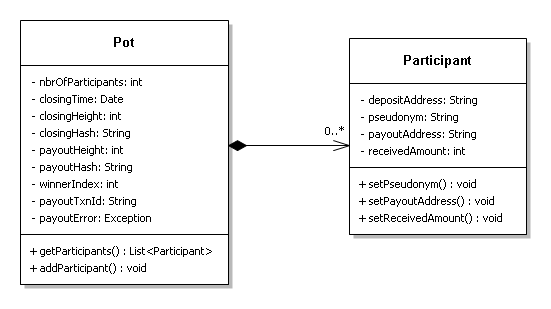
\includegraphics[width=1\linewidth]{Figures/umsetzung_btc/btc_datenmodell}
\decoRule
\caption{Java Datenmodel Klassendiagramm}
\label{fig:btc_datenmodell}
\end{figure}
\todo{private payoutStarted: boolean zur Klasse Pot hinzufügen.}

\subsection{Geschäftslogik}

Die Java Klassen der Glücksspielanwendung können, wie in Abbildung \ref{fig:btc_businesslogic} gezeigt, in 3 verschiedene Gruppen unterteilt werden. Das \textbf{Core Module} enthält die Klassen des Datenmodells und ein Interface mit dem die GUI Anwendung interagiert. Das Interface entkoppelt die Anzeigelogik der GUI von der Geschäftslogik der Kryptowährung. Die GUI Komponente bekommt von der Schnittstelle allgemeine Daten und kümmert sich nur um deren Anzeige.
Das \textbf{Bitcoin Service Module} enthält die gesamte kryptowährungsspezifische Geschäftslogik. \textbf{BitcoinJ} enthält alle Klassen und Interfaces die benötigt werden um mit dem Bitcoin Netzwerk zu interagieren und Daten aus der Blockchain auszulesen.

\begin{figure}[H]
\centering
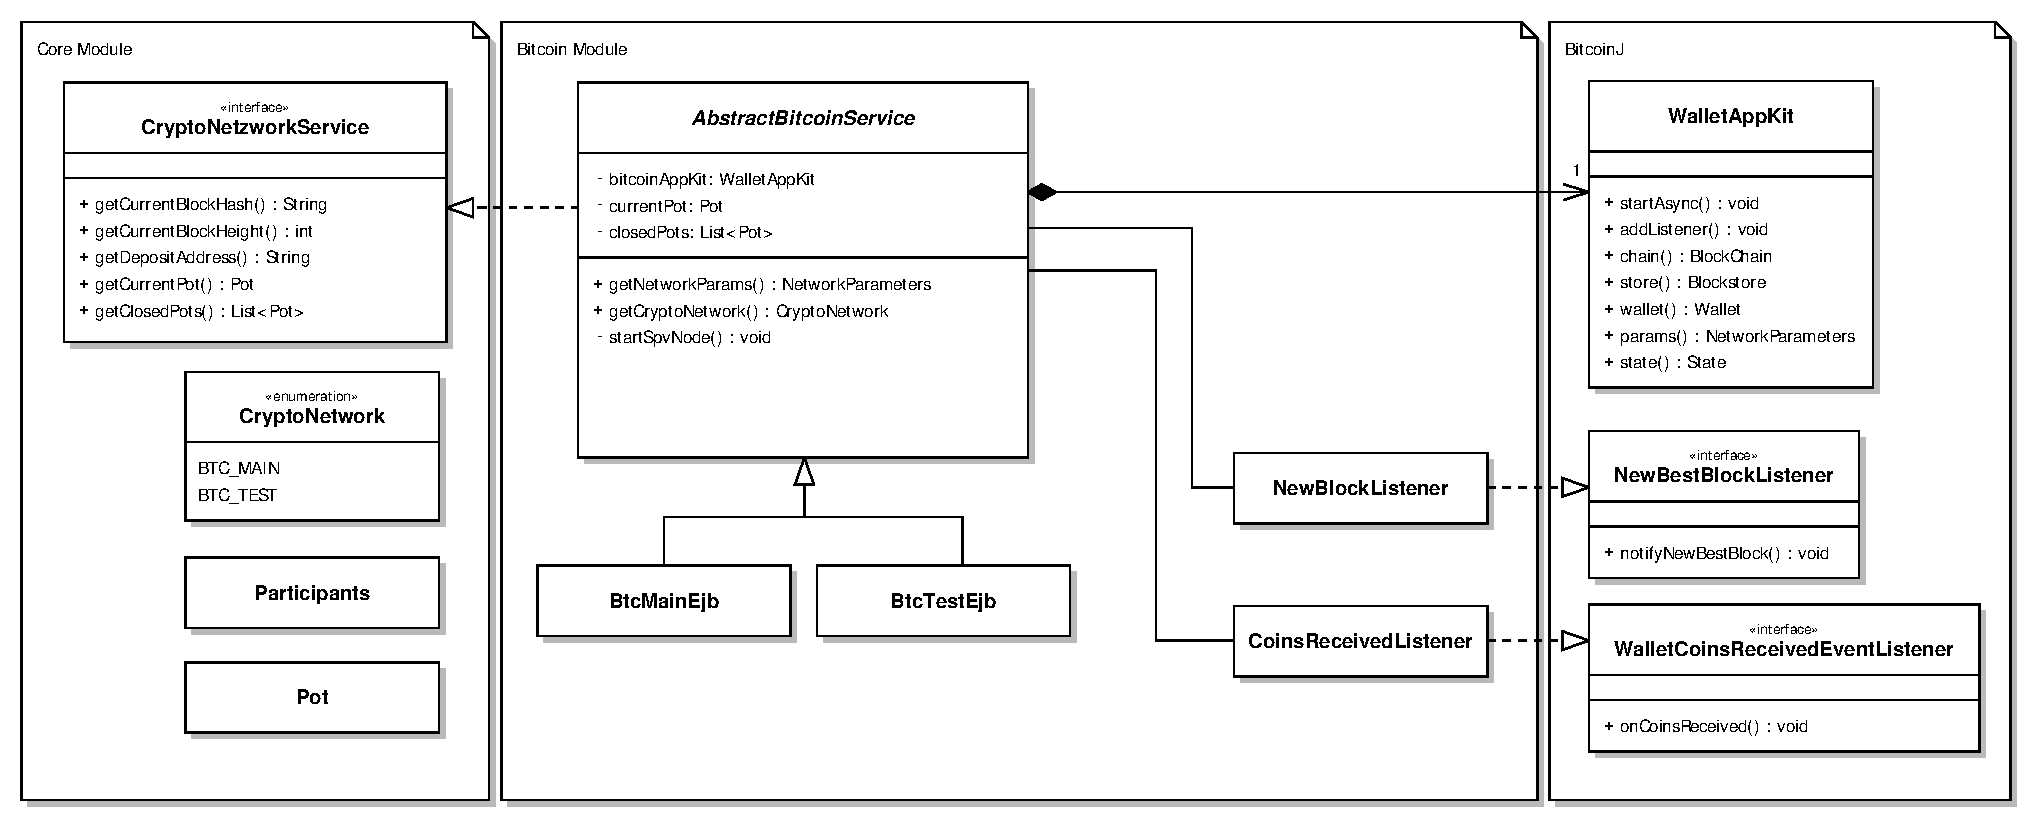
\includegraphics[width=1\linewidth]{Figures/umsetzung_btc/btc_businesslogic_pdf}
\decoRule
\caption{Java Geschäftslogik Klassendiagramm}
\label{fig:btc_businesslogic}
\end{figure}

\subsubsection{Start der Anwendung}
Beim Kompilieren der Anwendung wird über einen Konfigurationseintrag festgelegt, ob die Anwendung mit dem Bitcoin Haupt- oder Testnetzwerk interagieren soll.
Für das Hauptnetzwerk wird die Java Klasse \code{BtcMainEjb} verwendet. Für das Testnetwerk wird die Klasse \code{BtcTestEjb} verwendet. Beide Klassen verwenden die gleiche Implementierung der abstrakten Oberklasse \code{AbstractBitcoinService}. Diese wiederum implementiert das von der GUI Komponente verwendete Interface \code{CryptoNetworkservice}.

\begin{lstlisting}
import javax.ejb.Singleton;
import javax.ejb.Startup;
import org.bitcoinj.params.AbstractBitcoinNetParams;
import org.bitcoinj.params.MainNetParams;
import com.ossel.gamble.bitcoin.services.AbstractBitcoinService;
import com.ossel.gamble.core.data.enums.CryptoNetwork;
/**
 * Class will be excluded for the testnet jar via the maven jar plugin.
 */
@Startup
@Singleton
public class BtcMainEjb extends AbstractBitcoinService {
    @Override
    public CryptoNetwork getCryptoNetwork() {
        return CryptoNetwork.BTC_MAIN;
    }
    @Override
    public AbstractBitcoinNetParams getNetworkParams() {
        return MainNetParams.get();
    }
}
\end{lstlisting}


Die beiden Klassen \code{BtcMainEjb} und \code{BtcTestEjb} sind mit den Annotationen\code{@Startup} und \code{@Singleton} annotiert. Es handelt sich um sogenannte \textbf{E}nterprise \textbf{J}ava \textbf{B}eans. Dies bedeutet, dass der Applikationsserver diese eigenständig verwaltet und genau eine Instanz der Klasse beim Start der Applikation erzeugt. Beim Start wird dann die mit \code{@PostConstruct} annotierte \code{startSpvNode} Methode aufgerufen und abgearbeitet. Diese konfiguriert und startet das \code{WalletAppKit}, welches die zentrale Klasse zur Interaktion mit der BitcoinJ Bibliothek darstellt.

\begin{lstlisting}[basicstyle=\small] %or \tiny or \small or \footnotesize etc.
@PostConstruct
private void startSvpNode() {
    log.info("#### Start Bitcoin SPV Node  ####");
    currentPot = new Pot(2, 100000L);
    File walletDir = CoreUtil.getWalletDirectory();
    NetworkParameters params = getNetworkParams();
    String fileName = "bitcoin-" + params.getPaymentProtocolId();
    bitcoinAppKit = new WalletAppKit(params, walletDir, fileName) {
        @Override
        protected void onSetupCompleted() {
            log.info("#### Bitcoin SPV Node started ####");
        }
    };
    bitcoinAppKit.startAsync();
    waitUntilStarted(bitcoinAppKit);
    newBlockListener = new NewBlockListener(this);
    bitcoinAppKit.chain().addNewBestBlockListener(newBlockListener);
    coinReceivedListener = new CoinsReceivedListener(this);
    bitcoinAppKit.wallet().addCoinsReceivedEventListener(coinReceivedListener);
}
\end{lstlisting}

 In Zeile 4 wird zunächst ein neuer leerer Topf mit 2 Teilnehmern erzeugt. Anschließend wird das \code{WalletAppKit} erzeugt. Dazu bekommt dieses die gewünschten Netzwerkparameter und den Pfad zum Dateisystem in dem \code{BitcoinJ} die Blockchain- und Wallet-Daten speichern soll. Zeile 14 startet den durch das \code{WalletAppKit} repräsentierten SPV-Node. Anschließend wird dem \code{WalletAppKit} noch ein \code{NewBlockListener} und ein \code{CoinsReceivedListener} hinzugefügt, um auf neue Blöcke und eingehende Zahlungen zu reagieren.

\subsubsection{GUI Events}

Der folgende Code zeigt die Implementierung der Methoden die von der GUI Komponente aufgerufen werden.
\begin{lstlisting}
public Pot getCurrentPot() {
    return currentPot.clone();
}
public String getDepositAddress() {
    return bitcoinAppKit.wallet().freshAddress(KeyPurpose.RECEIVE_FUNDS).toString();
}
public String getCurrentBlockHash() {
    return bitcoinAppKit.chain().getChainHead().getHeader().getHash().toString();
}
public int getCurrentBlockHeight() {
    return bitcoinAppKit.chain().getChainHead().getHeight();
}
\end{lstlisting}


Die Methode \code{getCurrentPot} reicht in Zeile 2 die Daten des Topfs an die GUI Komponente weiter. Zeile 6 erzeugt eine neue Empfangsadresse und fügt einen weiteren möglichen Teilnehmer mit dieser Adresse der \code{possibleParticipants} Liste hinzu. Erst wenn eine Zahlung auf diese Adresse eingeht wird der Teilnehmer dem Topf hinzugefügt. Zeile 13 gibt den Blockhash des neusten Blocks der SPV Blockheader Kette zurück. Zeile 17 gibt die Blocknummer des neusten Blocks der SPV Blockheader Kette zurück.

\subsubsection{Bitcoin Netzwerk Events}

Immer wenn der SVP Node eine Transaktion auf eine vorher mittels der\\ \code{bitcoinAppKit.wallet().freshAddress()} erzeugten Adresse empfängt, wird die \code{onCoinsReceived} Methode der Klasse \code{CoinsReceivedListener} aufgerufen.

\begin{lstlisting}[basicstyle=\small]
@Override
public void onCoinsReceived(Wallet wallet, Transaction txn, Coin prevBalance, Coin newBalance) {
  log.debug("Transaction details: " + txn.toString());
  Coin value = txn.getValueSentToMe(wallet);
  Pot currentPot = service.getCurrentPot();
  if (currentPot.getExpectedBettingAmount() > value.getValue()) {
    log.warn("Player did not pay enough.");
    return;
  }
  List<Participant> participants = service.getPossibleParticipants();
  NetworkParameters params = service.getAppKit().params();
  for (TransactionOutput txnOutput : txn.getOutputs()) {
    Address a = txnOutput.getAddressFromP2PKHScript(params);
    String address = a.toString();
    for (Participant participant : participants) {
      String depositAddress = participant.getDepositAddress();
      if (depositAddress.equals(address)) {
        log.info("Received " + value.toFriendlyString() + " coins from " + participant.toString());
        participant.setReceivedAmount(value.getValue());
        String fromAddress = txn.getInput(0).getFromAddress().toString();
        participant.setPayoutAddress(fromAddress);
        wallet.addTransactionConfidenceEventListener(new TxnConfidenceListener(service, txn, participant));
      }
    }
  }
}
\end{lstlisting}


Zunächst wird in Zeile 6 geprüft, ob der eingegangene Zahlungsbetrag mindestens so hoch ist, wie von aktuellen Topf gefordert. Ist dies der Fall, iteriert die Methode über die Output Adressen\footnote{Eine detaillierte Beschreibung wie Bitcoin Transaktionen aufgebaut sind, liefert \cite{understanding_btc_txn}.} der Transaktion (Zeile 12) und prüft mit welcher Einzahlungsadresse der Teilnehmer (Teile 17) diese übereinstimmt. Handelt es sich bei der Output Adresse um keine Einzahlungsadresse eines Teilnehmers, wird diese ignoriert, da es sich um die Wechselgeldadresse eines Teilnehmers handeln muss\footnote{Bei Bitcoin können die einer Adresse zugewiesenen Währungseinheiten entweder ganz oder gar nicht ausgegeben werden. Daher ist es üblich eine vom Wallet kontrollierte Wechselgeldadresse in jeder Transaktion anzugeben.}. Hat man den Teilnehmer identifiziert, wird aus der Transaktion die Auszahlungsadresse berechnet und dem Teilnehmer der empfangene Geldbetrag gutgeschrieben (Zeile 19-21). Da es sich um eine gültige jedoch noch unbestätigte Transaktion handelt, wird der Teilnehmer erst nachdem die Transaktion in einen gültigen Block aufgenommen wurde zum Topf hinzugefügt. Zeile 22 erzeugt einen \code{TxnConfidenceListener} der diese Aufgabe übernimmt.

\begin{lstlisting}[basicstyle=\small]
@Override
public void onTransactionConfidenceChanged(Wallet wallet, Transaction txn) {
  if (txn.equals(targetTxn)) {
    log.debug("onTransactionConfidenceChanged Tx: " + txn.getHash());
    switch (txn.getConfidence().getConfidenceType()) {
      case PENDING:
        // unconfirmed but should be included shortly
        break;
      case BUILDING:
        // transaction is included in the best chain
        Pot currentPot = service.getCurrentPot();
        participant.setPotIndex(currentPot.getNbrOfParticipants());
        currentPot.addParticipant(participant);
        if (currentPot.isFull()) {
          service.closeCurrentPot(new Date());
        }
        wallet.removeTransactionConfidenceEventListener(this);
        break;
      case IN_CONFLICT:
        log.warn("possible double spend of txn " + txn.getHashAsString());
        break;
      case DEAD:
        log.warn("txn " + txn.getHashAsString()+ " won't confirm unless there is another re-org");
        wallet.removeTransactionConfidenceEventListener(this);
        break;
    }
  }
}
\end{lstlisting}


Die \code{onTransactionConfidenceChanged} Methode wird jedes mal aufgerufen wenn dem SPV-Client neue Daten zur Transaktion vorliegen. BitcoinJ unterscheidet zwischen vier verschiedenen \code{ConfidenceTypes}:
\begin{itemize}
\item PENDING: Bedeutet, dass die Transaktion noch unbestätigt ist und der SPV-Client darauf wartet, dass er einen Block erhält in dem die Transaktion enthalten ist.
\item BUILDING: Bedeutet, dass die Transaktion bereits in die Blockchain aufgenommen wurde. Durch den Aufruf von\\ \code{transaction.getConfidence().getAppearedAtChainHeight()} kann man abfragen, wie tief die Transaktion bereits in der Blockchain steckt. Diese Methode gibt zurück, wie viele Blöcke bereits auf den Block, der die Transaktion enthält, aufbauen. Die Glücksspielanwendung betrachtet eine Transaktion ab dem Zeitpunkt als final, ab dem sie in einen gültigen Block aufgenommen wurde.\footnote{Vor der Auszahlung des Gewinns kann die Anwendung erneut nachprüfen, ob es eine Restrukturierung der Blockchain durch einen Blockchainfork gab. Dadurch stellt sie sicher, dass alle Transaktionen Teil der längsten Blockkette geworden sind.} Geschieht dies, wird der Teilnehmer der Transaktion in den Topf hinzugefügt. \todo{Methode in COde einbauen unter BUILDING und dort über konfigurationswert festlegbar machen ab wann man die TXN akzeptiert.}
\item IN CONFLICT: In diesem Fall hat der SPV-Client zwei Transaktionen erhalten, die versuchen den gleichen Transaction-Output auszugeben. Man spricht von einem sogenannten ''double spend'' Angriff. 
\item DEAD: Transaktionen die diesen Status erhalten, können nicht mehr bestätigt werden, außer es kommt zu einer Blockchain Restrukturierung.\todo{Kann dieser Status wirklich vorkommen?}
\end{itemize}

Immer wenn der SVP Node einen neuen besten Block empfängt, den er vorne an die Blockheader Kette anhängen kann, wird die \code{notifyNewBestBlock} Methode aufgerufen.
\begin{lstlisting}[basicstyle=\small]
@Override
public void notifyNewBestBlock(StoredBlock block) throws VerificationException {
    log.info("New Block height = " + block.getHeight() + " hash = "
            + block.getHeader().getHash().toString());
    List<Pot> unfinishedPots = getUnfinishedPots(service.getClosedPots());
    for (Pot pot : unfinishedPots) {
        long potId = pot.getCreateTime().getTime();
        int payoutBlockHeight = pot.getPayoutBlockHeight();
        if (payoutBlockHeight > block.getHeight()) {
            log.info("Pot[" + potId + "] can not be handled yet.");
        } else if (payoutBlockHeight == block.getHeight()) {
            log.info("Pot[" + potId + "] select temorary Winner.");
            Block tmpPayoutBlock = new ExtendedBlock(block.getHeader().getHash().toString());
            pot.setPayoutBlock(tmpPayoutBlock);
            selectWinner(pot, tmpPayoutBlock);
        } else {
            log.info("Pot[" + potId + "] select final winner.");
            try {
               StoredBlock correctBlock = getPastBlock(payoutBlockHeight, block);
               String payoutBlockHash = correctBlock.getHeader().getHash().toString();
               Block finalPayoutBlock = new ExtendedBlock(payoutBlockHash);
               pot.setPayoutBlock(finalPayoutBlock);
               Participant winner = selectWinner(pot, finalPayoutBlock);
               log.info(winner.getDepositAddress() + " wins pot[" + potId + "].");
               startPayoutThread(pot);
            } catch (BlockStoreException e) {
               log.info("Couldn't select final winner of Pot[" + potId + "]:" + e.getMessage(), e);
            }
        }
    }
}
\end{lstlisting}



Diese Methode iteriert über alle bereits geschlossenen Töpfe, für die noch keine Auszahlung stattgefunden hat und unterscheidet dabei 3 Fälle:
\begin{enumerate}
\item Die Blocknummer des neusten Blocks ist kleiner als die Blocknummer, die den Topf entscheidet. In diesem Fall passiert nichts.
\item Der neue Block entscheidet den Topf, da die Blocknummer des Blocks gleich der \code{PayoutHeigth} des Topfs ist. Der Gewinner des Topfs wird selektiert, es findet allerdings keine Auszahlung statt. Die finale Auszahlung findet aus Sicherheitsgründen erst im nächsten Fall statt.
\item In diesem Fall gibt es mindestens einen Block, der auf dem Payout-Block des Topfs aufbaut. Ab diesem Zeitpunkt betrachtet die Anwendung den Gewinner als final.\footnote{An dieser Stelle kann man natürlich auch aus Sicherheitsgründen noch mehrere Blöcke abwarten, bevor die Anwendung eine Auszahlung startet. Ab einer Tiefe von 6 Blöcken gelten Bitcoin Zahlungen als irreversibel. Bei sehr hohen Zahlungen ist es empfehlenswert so lange abzuwarten.} Daher wird der Gewinner des Topfs überschrieben und die Auszahlung in einem neuen \code{Thread} gestartet.
\end{enumerate}

Die Klasse \code{ExtendedBlock} teilt den Blockhash zur Anzeige in der GUI in die Werte \code{perfix}, \code{lastDigit} und \code{suffix}. Die Variable \code{lastDigit} speichert die letzte numerische Stelle des Blockhashs und wird zur Gewinnerauswahl verwendet.

\begin{lstlisting}[basicstyle=\small]
public class ExtendedBlock extends Block {

    private String prefix;
    private String suffix;

    public ExtendedBlock(String blockHash) {
        super(blockHash, -1);
        int position = blockHash.length() - 1;
        while (position > 0) {
            char c = blockHash.charAt(position);
            int value = (int) c;
            if (value >= 48 && value <= 57) {// numeric
                this.lastDigit = Integer.parseInt(String.valueOf(c));
                break;
            }
            position--;
        }
        this.prefix = blockHash.substring(0, position);
        this.suffix = blockHash.substring(position + 1, blockHash.length());
    }
}
\end{lstlisting}







\subsubsection{Auszahlungen}
Auszahlung werden in einem eigenen Thread abgehandelt. Die Klasse \code{PayoutThread} ruft dazu die \code{payout} Methode auf.
\begin{lstlisting}
private void payout(Pot pot) throws InsufficientMoneyException, InterruptedException, ExecutionException {
    if (pot.isPayoutStarted()) {
        log.error("Payout already started: " + pot.getPayoutTxnId() + " - "
                + pot.getPayoutError());
    } else {
        pot.setPayoutStarted(true);
        Address winnerAddress = new Address(bitcoinService.getNetworkParams(),
                pot.getWinner().getPayoutAddress());
        Coin potValue = Coin.SATOSHI
                .multiply(pot.getParticipants().size() * pot.getExpectedBettingamount());
        Wallet.SendResult result = bitcoinService.getAppKit().wallet()
                .sendCoins(bitcoinService.getAppKit().peerGroup(), winnerAddress, potValue);
        String txnId = result.tx.getHash().toString();
        pot.setPayoutTxnId(txnId);
        log.info("Payout TXN ID = " + txnId);
        Transaction transaction = result.broadcastComplete.get();
        log(transaction);
    }
}
\end{lstlisting}


Die Methode prüft zunächst, dass die Auszahlung noch nicht gestartet wurde. Ist dies der Fall, wird der auszuzahlende Betrag berechnet und an die Adresse des Gewinners überwiesen. Anschließen wird die ID der Auszahlungstransaktion in den Topf geschrieben. Während der Auszahlung können von BitcoinJ 3 verschiedene Fehler auftreten:
\begin{enumerate}
\item InsufficientMoneyException: Falls die von der Wallet verwalteten Adressen nicht genug Bitcoin für die Auszahlung besitzen.
\item InterruptedException: Falls der Java Thread unterbrochen wird.
\item ExecutionException: Falls es zu einem unerwarteten Fehler bei der Ausführung kommt.
\end{enumerate}
Sollte es bei der Auszahlung ein Problem geben, wird die Exception gefangen und im \code{Pot} Objekt unter \code{payoutError} abgespeichert.

\subsection{Grafische Benutzeroberfläche}\label{ssec:btc_gui}

Die graphische Oberfläche der Anwendung ist mit dem Tapestry Framework von Apache realisiert. Da die GUI Komponente nur die Daten visualisiert, wird an dieser Stelle auf eine genauere Betrachtung verzichtet und lediglich die Benutzeroberfläche gezeigt.


\begin{figure}[H]
\centering
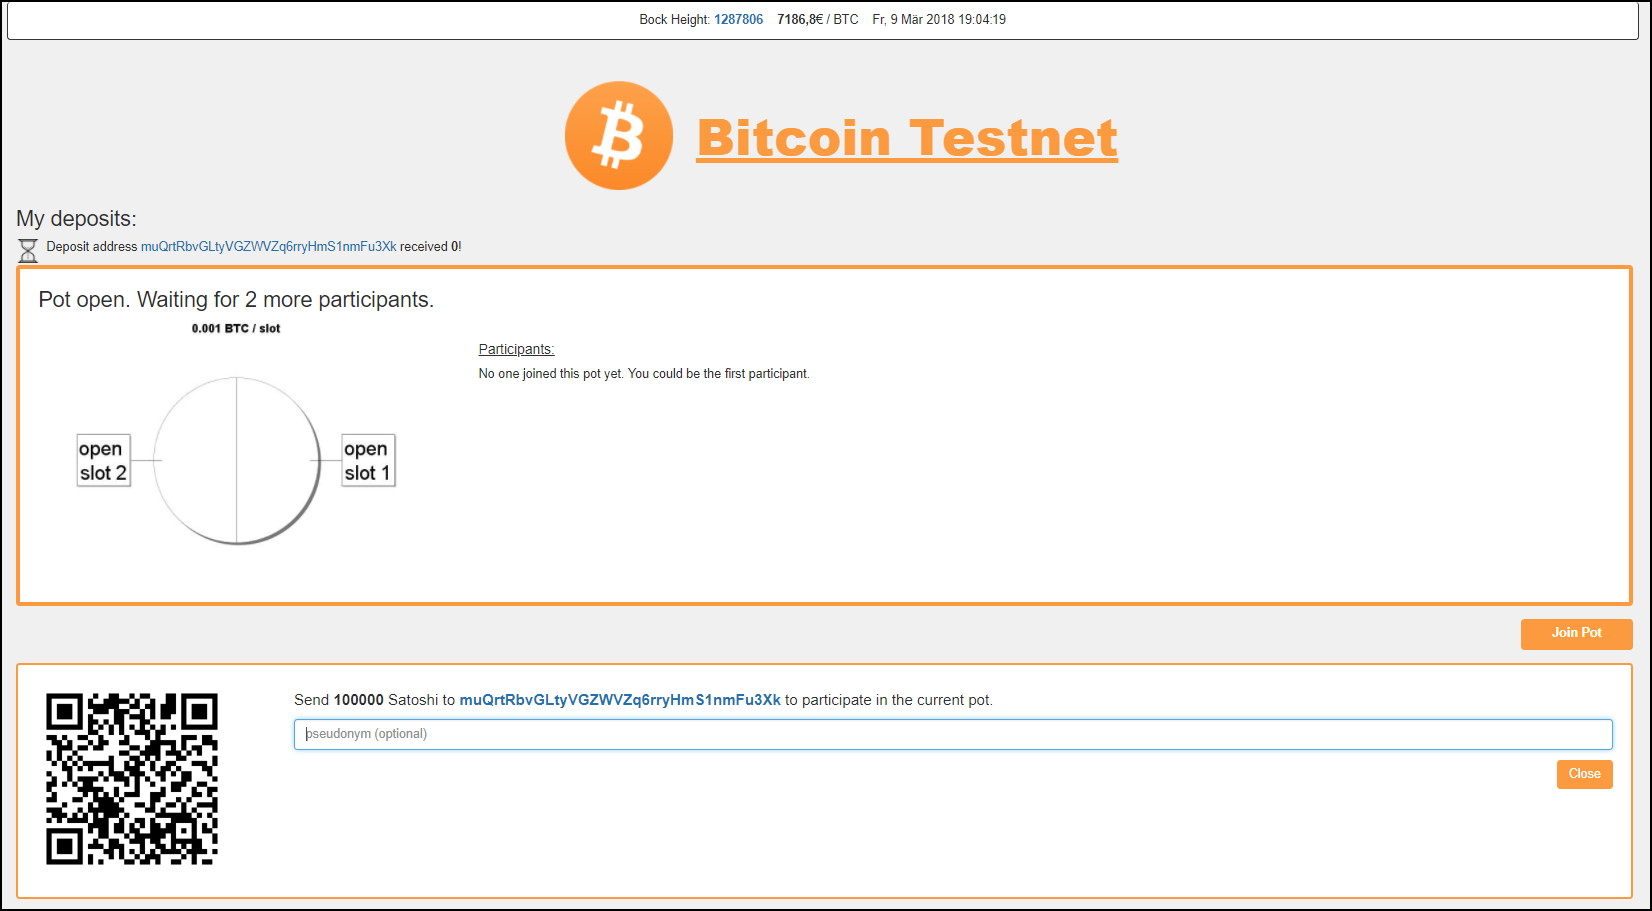
\includegraphics[width=1\linewidth]{Figures/btc_gui/pot_open_empty}
\decoRule
\caption{Leerer Topf}
\label{fig:pot_open_empty}
\end{figure}
Abbildung \ref{fig:pot_open_empty} zeigt einen Topf mit 2 freien Plätzen. Um dem Spiel beizutreten, muss der Spieler den Betrag von 0,001 Bitcoin an die angezeigte Adresse senden. Der angezeigte QR-Code erleichtert dem Spieler die Übertragung dieser Daten in das Überweisungsformular seines Smartphone Wallets. Das \textbf{B}itcoin \textbf{I}mprovement \textbf{P}roposal Nummer 21 \cite{bip21} legt fest, in welchem Format diese Daten kodiert werden müssen, damit beliebige Bitcoin Clients diese auslesen und interpretieren können. 
Folgende Daten sind in dem QR Code enthalten:\\ ''bitcoin:muQrtRbvGLtyVGZWVZq6rryHmS1nmFu3Xk?amount=0.001''

\vspace{1cm}
\begin{minipage}{0.48\textwidth}
\begin{figure}[H]
\centering
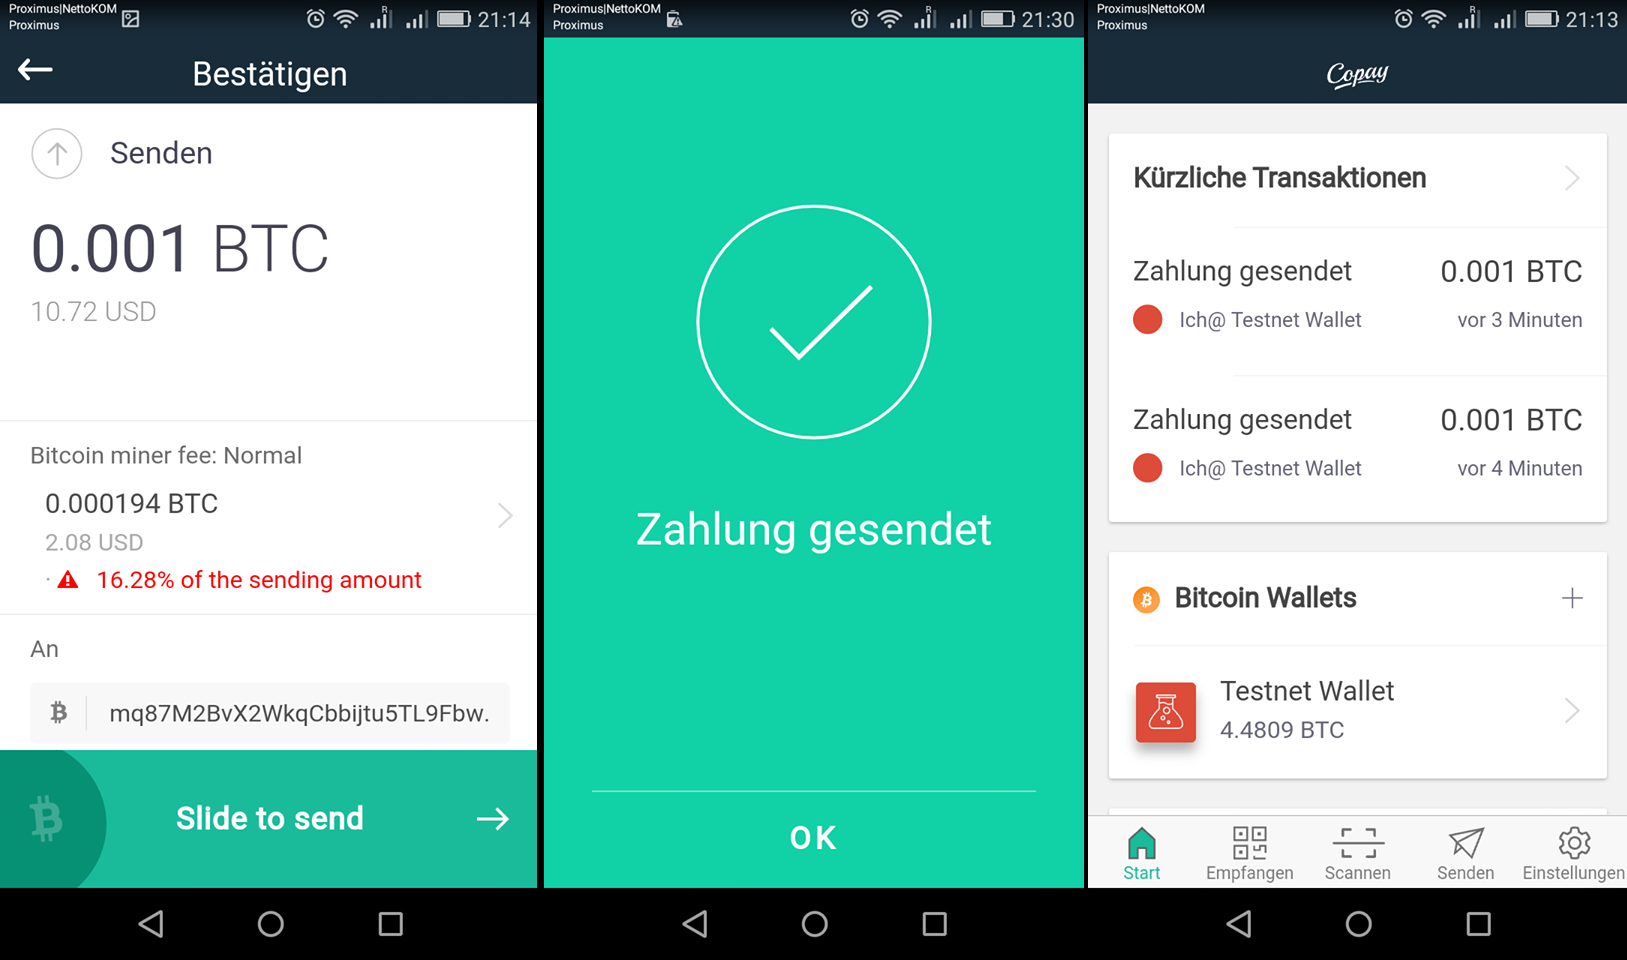
\includegraphics[width=1\linewidth]{Figures/btc_gui/handy_send}
\decoRule
\caption{Smartphone Überweisungsformular}
\label{fig:handy_send}
\end{figure}
\end{minipage}
\begin{minipage}{0.48\textwidth}
\begin{figure}[H]
\centering
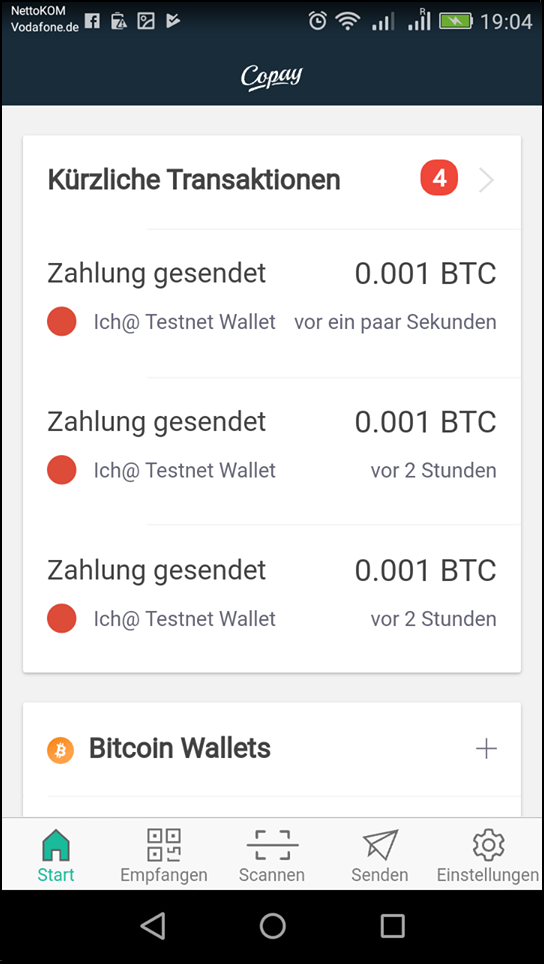
\includegraphics[width=1\linewidth]{Figures/btc_gui/handy_confirm}
\decoRule
\caption{Zahlungsbestätigung}
\label{fig:handy_confirm}
\end{figure}
\end{minipage}

Abbildungen \ref{fig:handy_send} und \ref{fig:handy_confirm} zeigen das Bitcoin CoPay Wallet\footnote{\url{https://copay.io/}}. Dieses erlautb, neben Zahlungen im Bitcoin Hauptnetzwerk, auch Zahlungen an das Bitcoin Testnetz zu senden. Nachdem der Benutzer den QR-Code der Glücksspielanwendung mit seinem Smartphone abgescannt hat, erscheint sowohl der Betrag als auch die Empfangsadresse vorausgefüllt im Überweisungsformular. Die Wallet berechnet automatisch eine passende Transaktionsgebühr. Der Spieler überprüft lediglich die Adresse und den Betrag und  autorisiert anschließend die Zahlung.

\begin{figure}[H]
\centering
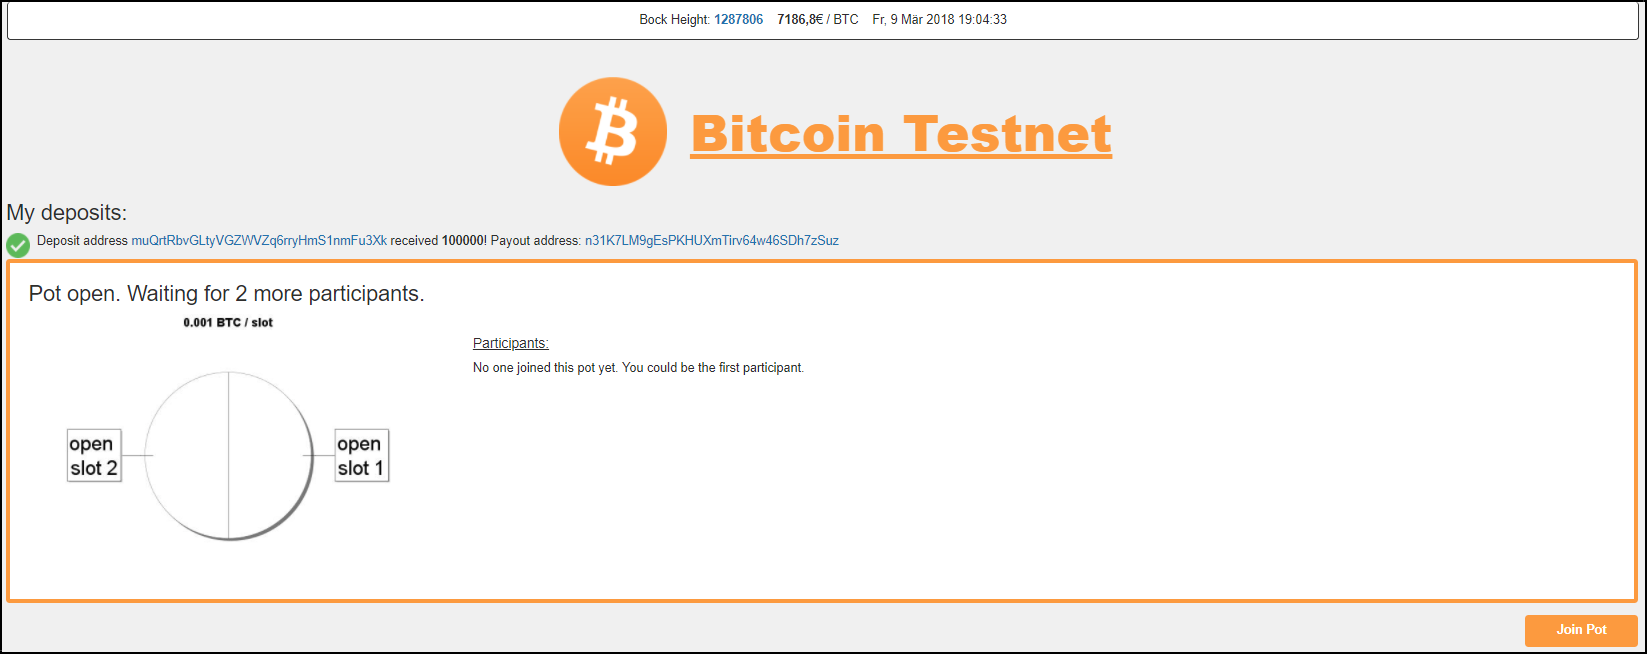
\includegraphics[width=1\linewidth]{Figures/btc_gui/pot_open_payment_received}
\decoRule
\caption{Transaktion empfangen}
\label{fig:pot_open_payment_received}
\end{figure}

Sobald die Anwendung die Transaktion empfängt, zeigt sie dies durch einen grünen Haken an. Dies ist in Abbildungen \ref{fig:pot_open_payment_received} zu sehen. Zu diesem Zeitpunkt handelt es sich um eine unbestätigte Transaktion, die noch in keinen Bock der Blockchain aufgenommen wurde.

\begin{figure}[H]
\centering
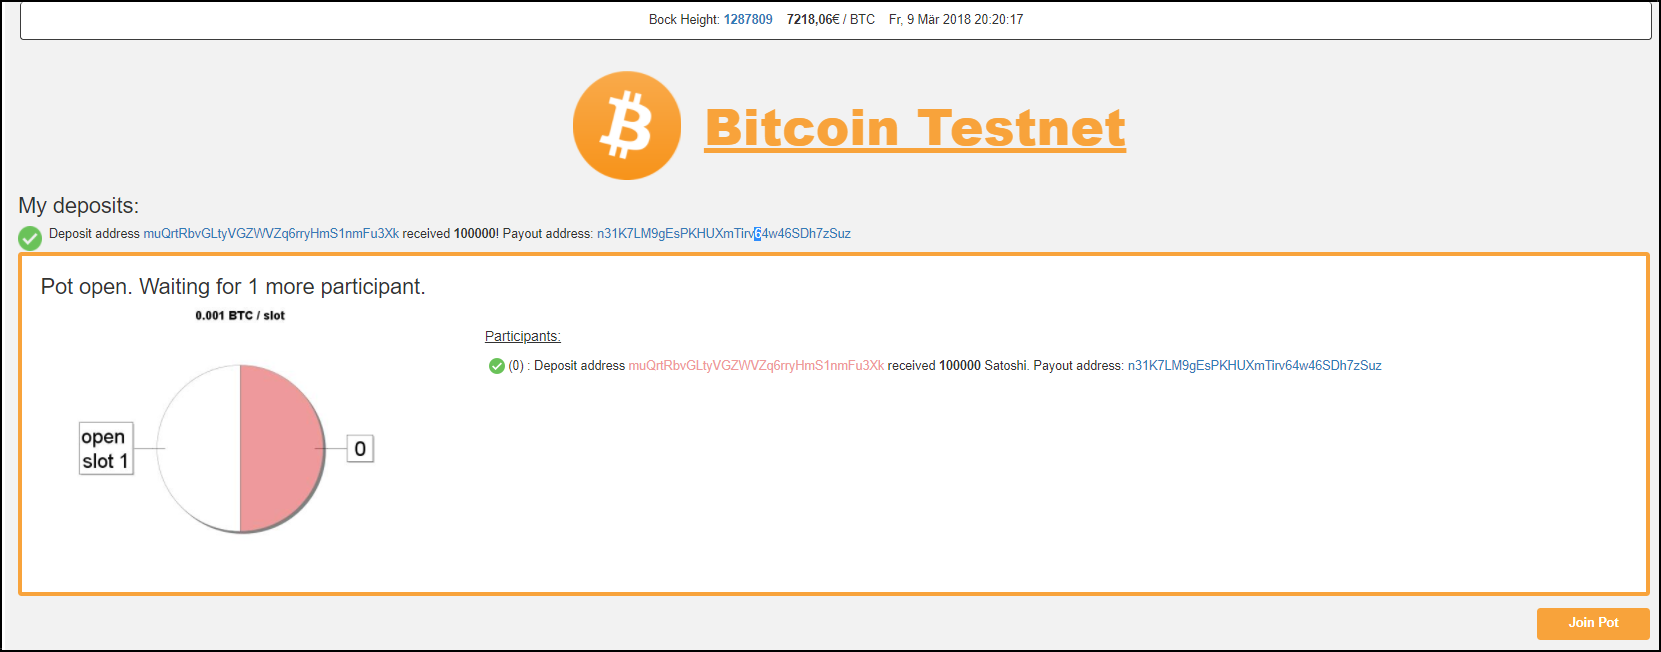
\includegraphics[width=1\linewidth]{Figures/btc_gui/pot_open_p1_confirmed}
\decoRule
\caption{Spieler zu Topf hinzugefügt.}
\label{fig:pot_open_p1_confirmed}
\end{figure}
Sobald die Anwendung einen neuen Block empfängt, der die Transaktion enthält, gilt die Transaktion als bestätigt und der Spieler wird zum Topf hinzugefügt. Nun gibt es nur noch einen offenen Platz im Topf.

\begin{figure}[H]
\centering
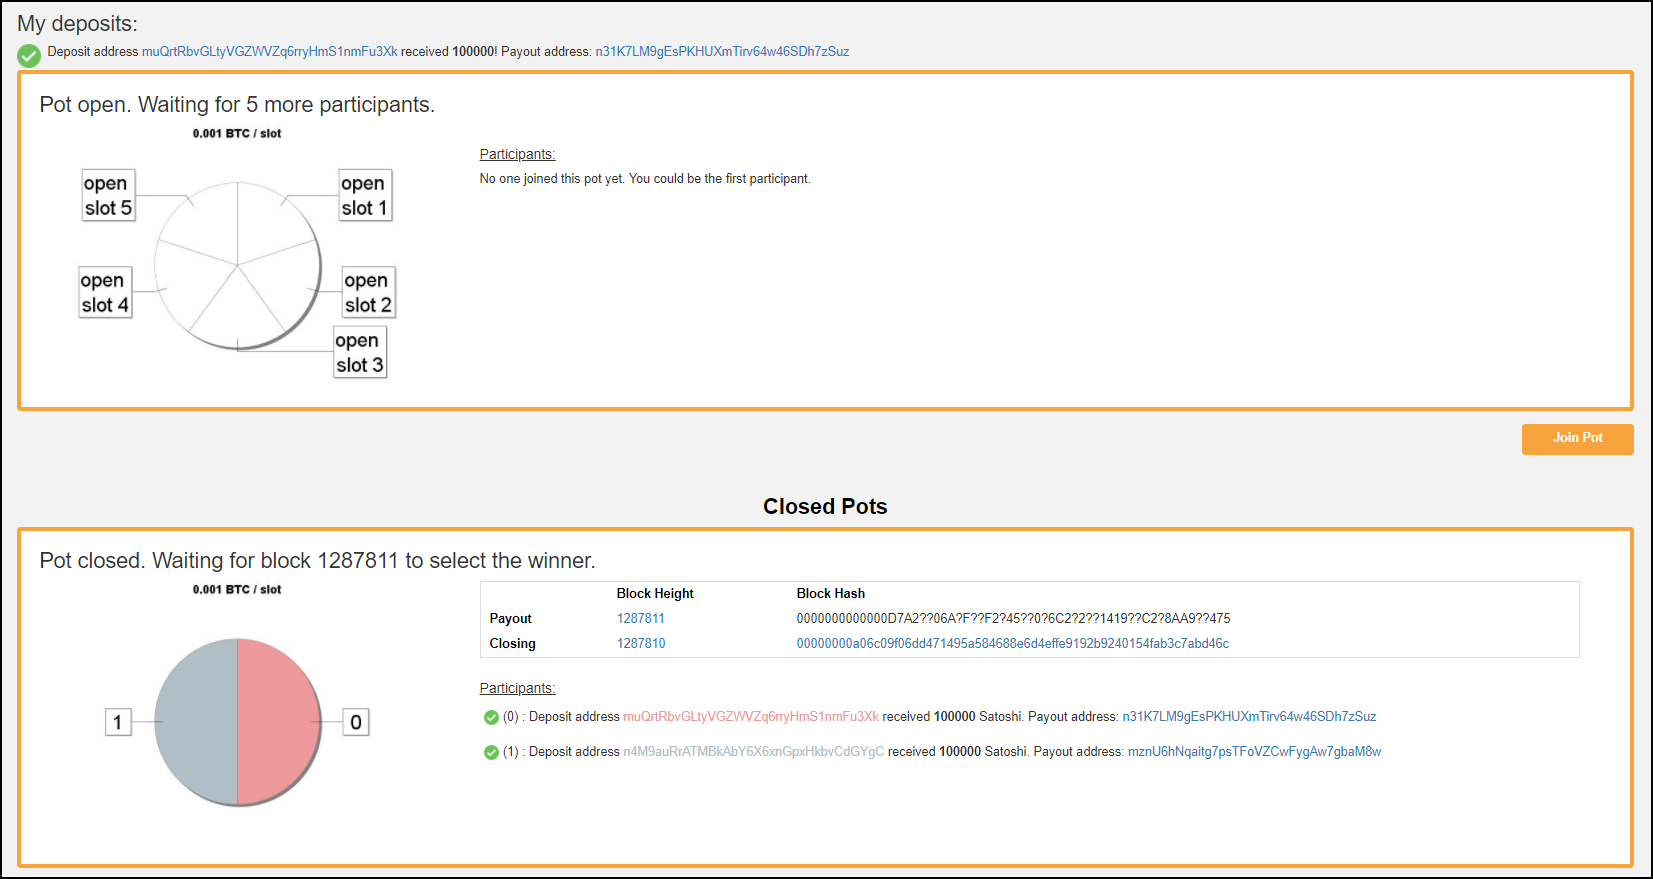
\includegraphics[width=1\linewidth]{Figures/btc_gui/pot_closed}
\decoRule
\caption{Topf geschlossen}
\label{fig:pot_closed}
\end{figure}

Nachdem ein weiterer Spieler in den Topf eingezahlt hat, ist der Topf voll. Die Anwendung schließt den aktuellen Topf und öffnet einen neuen Topf. Die Anwendung erstellt zufällig entweder einen Topf mit 2, 5 oder 10 freien Plätzen. In einer real eingesetzten Glücksspielanwendung würden alle Spielvarianten parallel angeboten. Der in Abbildung \ref{fig:pot_closed} gezeigte neue Topf hat fünf freie Plätze. Die Anwendung wartet nun auf den \code{Payout}-Block, um den Gewinner des geschlossenen Topfs festzulegen. Da der Blockhash noch nicht feststeht, zeigt die Anwendung die Animation eines sich sehr schnell wechselnden Blockhashs an, der mehrere Fragezeichen enthält.

\begin{figure}[H]
\centering
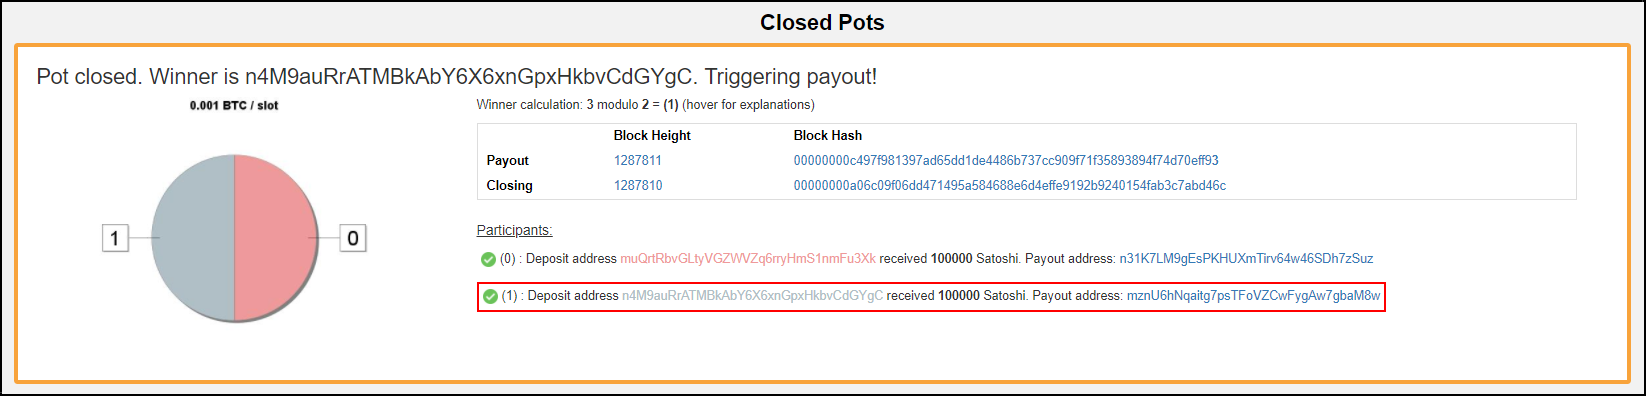
\includegraphics[width=1\linewidth]{Figures/btc_gui/pot_closed_triggering_payout}
\decoRule
\caption{Gewinner ermittelt}
\label{fig:pot_closed_triggering_payout}
\end{figure}
Sobald der entscheidende Block empfangen wird, wird der voraussichtliche Gewinner des Topfs durch ein rotes Rechteck markiert. Außerdem zeigt die Anwendung durch welche Berechnung der Gewinner festgelegt wurde. Nun wartet die Anwendung bis ein weiterer Block gefunden wird, bevor sie die Auszahlung an den Gewinner startet. 

\begin{figure}[H]
\centering
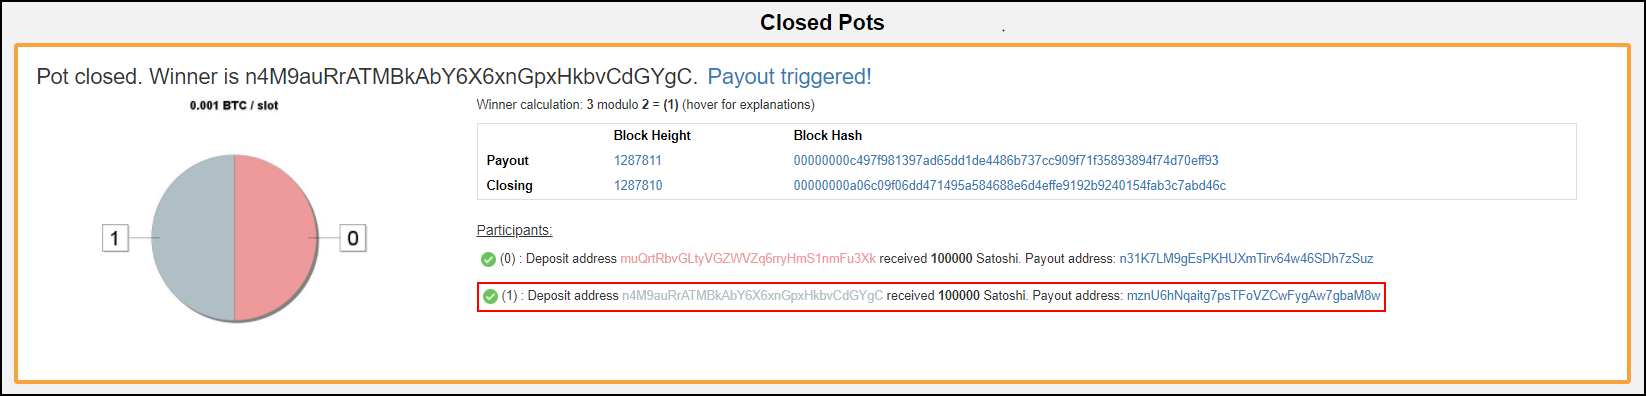
\includegraphics[width=1\linewidth]{Figures/btc_gui/pot_closed_payout_finished}
\decoRule
\caption{Auszahlung beendet}
\label{fig:pot_closed_payout_finished}
\end{figure}

Klickt der Benutzer auf den \emph{Payout triggered} Link aus Abbildung \ref{fig:pot_closed_payout_finished}, gelangt er zu einem Blockexplorer. Dieser zeigt ihm die Transaktionsdetails an. Eine genauere Betrachtung findet in Abschnitt \ref{sssec:Auszahlungstransaktion} statt.